
\chapter{Aplikace v konkrétních rodinách distribucí}

V této kapitole použijeme minimální Rényiho odhady ($\mathfrak{R}_\alpha$-odhady) v různých rozděleních pravděpodobnosti. Výsledky pro normální rozdělení byly uvedeny již v \cite{Demut2010}. My jsem se tedy zaměřili na exponenciální, Laplaceovo, Cauchyho a Weibullovo rozdělení pravděpodobnosti. V případě těchto rodin jsme se snažili o odvození konkrétního tvaru odhadu podle \eqref{Renyi-estimator_formula} a také tvaru influeční funkce \eqref{IF}.

\section{Laplaceovo rozdělení} %%%%%%%%%%%%%%%%%%%%%  LAPLACE   %%%%%%%%%%%%%%%%%%%%%%

Zde použijeme minimální $\mathfrak{R}_\alpha$-odhady k odhadu parametru $\theta = (\mu,\lambda)$ pro případ Laplaceova rozdělení. Hustota pravděpodobnosti má tedy tvar
\begin{equation}
	p_\theta = \frac{1}{2\lambda} e^{-\frac{|x-\mu|}{\lambda}}, \qquad \mu\in \mathbb{R},\, \lambda>0.
\end{equation}
Pro $\alpha = 0$ se odhad podle \eqref{Renyi-estimator_formula} rovná maximálně věrohodnému odhadu
\begin{eqnarray}
	\hat{\theta}_{\mathfrak{R}_\alpha,n} & = & \arg \max_{\theta \in \Theta} \frac{1}{n} \sum^n_{i=1} \ln \left[ \frac{1}{2\lambda}\exp \left[-\frac{|x_i-\mu|}{\lambda} \right] \right] \nonumber \\
	& = & \arg \max_{\theta \in \Theta} \left[ \ln \frac{1}{2\lambda} - \frac{1}{n} \sum^n_{i=1} \frac{|x_i-\mu|}{\lambda} \right].
\end{eqnarray}
Podmínka \ref{beta-podminka} platí pro každé $\beta>0$, takže pak pro $\alpha>0$ můžeme  min $\mathfrak{R}_\alpha$-odhad \eqref{Renyi-estimator_formula} pro Laplaceovo rozdělení psát jako 
\begin{equation}
	\hat{\theta}_{\mathfrak{R}_\alpha,n} = \arg \max_{\theta \in \Theta} \left[ (2\lambda)^{-\frac{\alpha}{1+\alpha}} \frac{1}{n} \sum_{i=1}^n \exp \left[-\alpha\frac{|x_i-\mu|}{\lambda} \right] \right].
	\label{renyi-formula-laplace}
\end{equation}

Nyní spočítáme influenční funkci podle \eqref{IF}. Položíme-li odhadovaný parametr $\theta = \mu$ při známém $\lambda$, pak nám vychází 

\begin{equation}
	\mathrm{IF}(x;T_{\mathfrak{R}_\alpha},\mu) = (1+\alpha )^{\frac{3}{2}} (x-\mu )  e^{-\frac{\alpha}{2} (x-\mu )^2}. % IF(x,mu)
	\label{IF-laplace-mu}
\end{equation}
Pokud prohodíme úlohu parametrů, tedy pokud bude hledaným parametrem $\theta = \lambda$ a $ \mu$ bude známe, vychází 
\begin{equation}
	\mathrm{IF}(x;T_{\mathfrak{R}_\alpha},\lambda) = (1 + \alpha)^2 \left(-\lambda + (1 + \alpha)|x-\mu|\right)  e^{-\frac{\alpha|x-\mu|}{\lambda}}	. % IF(x,sigma)
	\label{IF-laplace-lambda}
\end{equation}

\begin{figure}[htb]
\begin{center}
\begin{tabular}{c c c}
	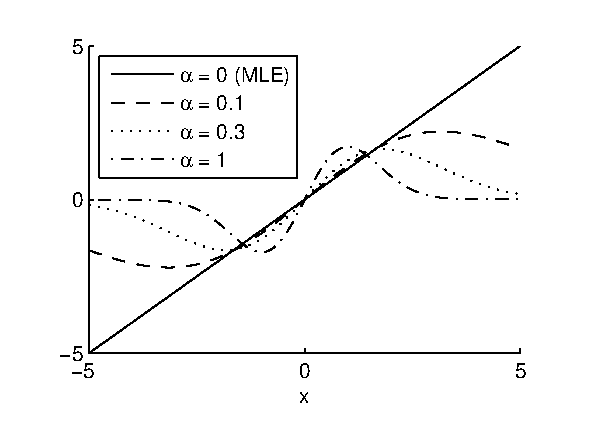
\epsfig{file=Laplace-IF-mu.eps, height=2.in} 
	&&
	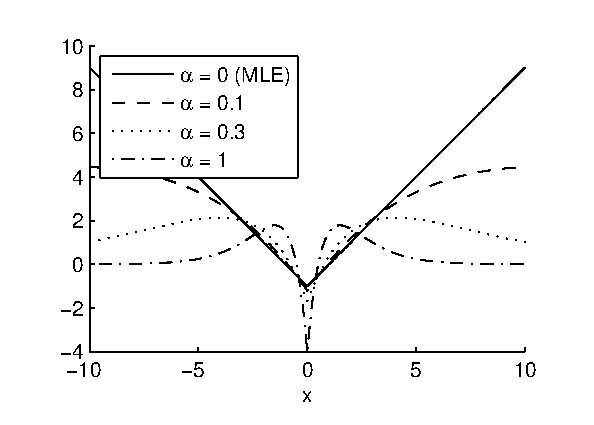
\epsfig{file=Laplace-IF-lambda.eps, height=2.in} 
	\\
	$\mathrm{IF}(x;T_{\mathfrak{R}_\alpha},\mu = 0) $ při známém $\lambda = 1$ 
	&&
	$\mathrm{IF}(x;T_{\mathfrak{R}_\alpha},\lambda = 1)$ při známém $\mu = 0$ 
	\\
\end{tabular}
\caption{Influenční funkce {\mRao}ů pro Laplaceovo rozdělení}
\end{center}
\label{fig:laplace-if}
\end{figure}

\noindent Z \eqref{IF-laplace-mu} a \eqref{IF-laplace-lambda} vidíme, že jsou obě influenční funkce pro $\alpha>0$ omezené, tedy B-robustní a navíc pro obě funkce platí

\begin{equation}
	\lim_{x \rightarrow \pm\infty} \mathrm{IF}(x;T_{\mathfrak{R}_\alpha},\cdot) = 0.
\end{equation}
 
\noindent Nemáme sice konečný bod zamítání $\rho^*$, ale influenční funkce se alespoň limitně blíží s rostoucím $x$ k nule. Tato konvergence je s větším $\alpha$ rychlejší kvůli členu $e^{-\alpha x}$, který se vyskytuje v obou funkcích.

\section{Exponenciální rozdělení} %%%%%%%%%%%%%%%%%%%%%  EXPONENTIAL   %%%%%%%%%%%%%%%%%%%%%%

Nyní použijeme minimální $\mathfrak{R}_\alpha$-odhady k odhadu parametru $\theta = (\mu,\lambda)$ pro případ exponenciálního rozdělení s hustotou pravděpodobnosti
\begin{equation}
	p_\theta = \frac{1}{\lambda} e^{-\frac{x-\mu}{\lambda}}, \qquad \mu\in \mathbb{R},\, \lambda>0, \, x>\mu.
\end{equation}
Pro $\alpha = 0$ je 
\begin{eqnarray}
	\hat{\theta}_{\mathfrak{R}_\alpha,n} & = & \arg \max_{\theta \in \Theta} \frac{1}{n} \sum^n_{i=1} \ln \left[ \frac{1}{\lambda}\exp \left[-\frac{x_i-\mu}{\lambda} \right] \right] \nonumber \\
	& = & \arg \max_{\theta \in \Theta} \left[ \ln \frac{1}{\lambda} - \frac{1}{n} \sum^n_{i=1} \frac{x_i-\mu}{\lambda} \right].
\end{eqnarray}

\noindent Podmínka \ref{beta-podminka} opět platí pro každé $\beta>0$, takže pak pro $\alpha>0$ můžeme  min $\mathfrak{R}_\alpha$-odhad \eqref{Renyi-estimator_formula} pro exponenciální rozdělení psát jako 

\begin{equation}
	\hat{\theta}_{\mathfrak{R}_\alpha,n} = \arg \max_{\theta \in \Theta} \lambda^{-\frac{\alpha}{1+\alpha}} \frac{1}{n}\sum_{i=1}^n \exp \left[-\alpha\frac{x_i-\mu}{\lambda} \right].
	\label{renyi-formula-exponential}
\end{equation}

\noindent Je vidět, že rozdíl oproti \eqref{renyi-formula-laplace} je jen v použití absolutní hodnoty u odhadu Laplaceova rozdělení. 

Influenční funkce je podle $\eqref{IF}$ v případě odhadovaného parametru $\theta = \mu$ a známého $ \lambda$ stejná jako pro Laplaceovo rozdělení $\eqref{IF-laplace-mu}$, tedy 

\begin{equation}
	\mathrm{IF}(x;T_{\mathfrak{R}_\alpha},\mu) = (1+\alpha )^{\frac{3}{2}} (x-\mu )  e^{-\frac{\alpha}{2} (x-\mu )^2}. % IF(x,mu)
	\label{IF-exponential-mu}
\end{equation}
Pokud naopak je hledaným parametrem $\theta = \lambda$ a $ \mu $ známe, vychází 
\begin{equation}
	\mathrm{IF}(x;T_{\mathfrak{R}_\alpha},\lambda) =	(1+\alpha )^2 \left( - \lambda +(1+ \alpha)(x-\mu)\right) e^{-\frac{\alpha (x-\mu)}{\lambda }} % IF(x,lambda),
	\label{IF-exponential-lambda}
\end{equation}

\begin{figure}[htb]
\begin{center}
\begin{tabular}{c c c}
	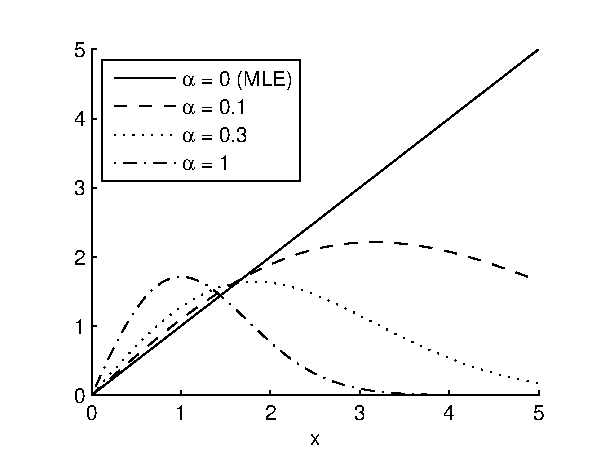
\epsfig{file=Exp-IF-mu.eps, height=2.1in} 
	&&
	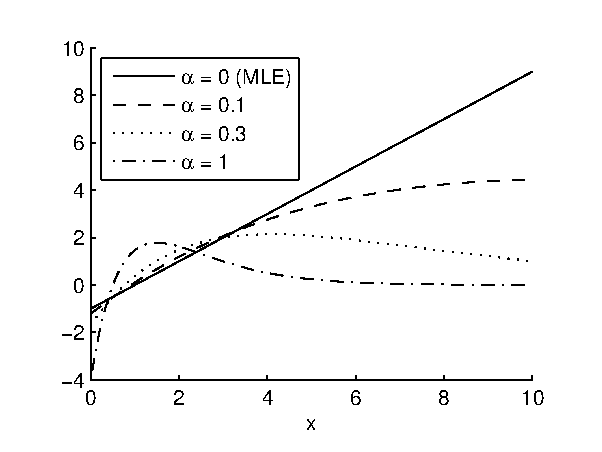
\epsfig{file=Exp-IF-lambda.eps, height=2.1in} 
	\\
	$\mathrm{IF}(x;T_{\mathfrak{R}_\alpha},\mu = 0) $ při známém $\lambda = 1$
	&&
	$\mathrm{IF}(x;T_{\mathfrak{R}_\alpha},\lambda = 1)$ při známém $\mu = 0$
	\\
\end{tabular}
\caption{Influenční funkce {\mRao}ů pro exponenciální rozdělení}
\end{center}
\label{fig:exponencialni-if}
\end{figure}

\noindent Z \eqref{IF-exponential-mu} a \eqref{IF-exponential-lambda} opět vidíme, že jsou obě influenční funkce pro $\alpha>0$ omezené, a opět pro obě funkce platí

\begin{equation}
	\lim_{x \rightarrow \pm\infty} \mathrm{IF}(x;T_{\mathfrak{R}_\alpha},\cdot) = 0.
\end{equation}
 
\noindent Přitom platí, že se konvergence kvůli členu $ e^{-\alpha x}$ zrychluje s rostoucím $\alpha$.

\section{Cauchyovo rozdělení} %%%%%%%%%%%%%%%%%%%%%  Cauchy   %%%%%%%%%%%%%%%%%%%%%%


Dalším rozdělením, na které jsme použili Rényiho odhady, je Cauchyovo rozdělení s parametrem $\theta = (\mu,\sigma)$ a hustotou pravděpodobnosti
\begin{equation}
	p_\theta = \frac{1}{\pi\sigma} \left( 1 + \left( \frac{x-\mu}{\sigma} \right)^2 \right)^{-1}, \qquad \mu\in \mathbb{R},\, \sigma>0.
\end{equation}
Pro $\alpha = 0$ je {\mRao} roven
\begin{eqnarray}
	\hat{\theta}_{\mathfrak{R}_\alpha,n} & = & \arg \max_{\theta \in \Theta} \frac{1}{n} \sum^n_{i=1} \ln \left[  \frac{1}{\pi\sigma} \left( 1 + \left( \frac{x_i-\mu}{\sigma} \right)^2 \right)^{-1}   \right] \nonumber \\
	& = & \arg \max_{\theta \in \Theta} \left[ -\ln \pi\sigma - \frac{1}{n} \sum^n_{i=1} \ln \left[ 1 + \left( \frac{x_i-\mu}{\sigma} \right)^2 \right] \right].
\end{eqnarray}
Ten už však není shodný s maximálně věrohodným odhadem, který má tvar
\begin{equation}
	\hat{\theta}_{\mathrm{MLE},n} = \arg \max_{\theta \in \Theta}  \ln \sum^n_{i=1} \frac{1}{\pi\sigma} \left[ 1 + \left( \frac{x_i-\mu}{\sigma} \right)^2 \right].
\end{equation}

\noindent Podmínka \ref{beta-podminka} opět platí pro každé $\beta>0$. Pro $\alpha>0$ pak vychází minimální $\mathfrak{R}_\alpha$-odhad \eqref{Renyi-estimator_formula} pro Cauchyovo rozdělení jako

\begin{equation}
	\hat{\theta}_{\mathfrak{R}_\alpha,n} = \arg \max_{\theta \in \Theta} \left[ \sigma^{-\frac{\alpha}{1+\alpha}} \frac{1}{n} \sum_{i=1}^n \left( 1 + \left( \frac{x_i-\mu}{\sigma} \right)^2 \right)^{-\alpha} \right].
	\label{renyi-formula-cauchy}
\end{equation}

Influenční funkci $\eqref{IF}$ se nám podařilo dopočítat jen pro neznámý parametr $\theta = \mu$. Influenční funkce má pak tvar

\begin{equation}
	\mathrm{IF}(x;T_{\mathfrak{R}_\alpha},\mu) = \sqrt{\pi}\frac{\Gamma\left( 3 + \alpha \right)}{\Gamma\left( \frac{3}{2} + \alpha \right)} \left( \frac{\sigma^2}{\sigma^2 + (x-\mu)^2}\right)^{1+\alpha}(x-\mu).
	\label{IF-cauchy-mu}
\end{equation}

\noindent Z \eqref{IF-cauchy-mu}je vidět, že influenční funkce je pro $\alpha>0$ omezená, a opět pro ni pro $\alpha>0$ platí

\begin{equation}
	\lim_{x \rightarrow \pm\infty} \mathrm{IF}(x;T_{\mathfrak{R}_\alpha},\mu) = 0.
\end{equation}

\begin{figure}[htb]
\begin{center}
\begin{tabular}{c}
	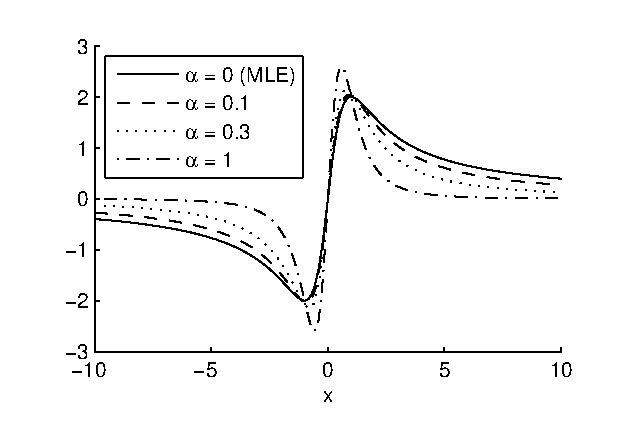
\epsfig{file=Cauchy-IF-mu.eps, height=2.6in} \\
	$\mathrm{IF}(x;T_{\mathfrak{R}_\alpha},\mu = 0) $ při $\sigma = 1$ známém
\end{tabular}
\caption{Influenční funkce {\mRao}ů pro Cauchyovo rozdělení}
\end{center}
\label{fig:cauchy-if}
\end{figure}

\noindent Pro neznámý parametr $\theta = \sigma$ vyšla influenční funkce po výpočtu ve \texttt{Wolphram Mathematica} ve tvaru

\begin{eqnarray}
&-\left[4 \sqrt{\pi } (1+\alpha )^2 \sigma ^{2+\alpha } \left(\frac{\sigma }{(x-\mu )^2+\sigma ^2}\right)^{\alpha } \left(\frac{1}{\sigma }+\frac{\alpha  \left(\frac{1}{\sigma }\right)^{\alpha } \sigma ^{-1+\alpha }}{1+\alpha }-\frac{2 \sigma }{(x-\mu )^2+\sigma ^2}\right) \right. \nonumber \\
&\left. \cos[\pi  \alpha ] \Gamma[\alpha ] \Gamma[1+\alpha ]  \frac{}{} \right] / \nonumber \\ %prázdný zlomek je tam kvůli roztažení koncové závorky
&\left(4^{1-\alpha } \sqrt{\pi } \left(\frac{1}{\sigma }\right)^{\alpha } \sigma ^{\alpha } \left(-1+\alpha  \left(-1+\alpha  \left(-2+\left(\frac{1}{\sigma }\right)^{\alpha } \sigma ^{\alpha }\right)\right)\right) \right.\nonumber \\ 
&\left. \cos[\pi  \alpha ] \Gamma[1+2 \alpha ]+1/(3 (3+4 \alpha  (2+\alpha )))\right. \nonumber \\
& 8 \pi  (1+\alpha ) \left(-1+\alpha  (1+\alpha )^2\right) \Gamma[\alpha ] \nonumber \\
&\left. \left(6 (1+\alpha ) ^r_2\mathrm{F}_1\left[\frac{1}{2},2,\frac{1}{2}-\alpha ,1\right]-4^{-\alpha } \Gamma[4+2 \alpha ] ^r_2\mathrm{F}_1\left[\frac{1}{2}+\alpha ,1+\alpha ,-\frac{1}{2}+\alpha ,1\right]\right)\right),
\end{eqnarray}

\noindent kde $^r_2\mathrm{F}_1[a,b;c;z]$ je regularizovaná hypergeometrická funkce 

\begin{equation}
	^r_2\mathrm{F}_1[a,b;c;z] = {\frac{1}{\Gamma[c]}} {_2\mathrm{F}_1}[a,b;c;z],
\end{equation}
\begin{equation}
	{_2\mathrm{F}_1}[a,b;c;z]=\sum _{k=0}^{\infty } \frac{(a)_k (b)_k z^k}{ (c)_k k!} \qquad |z|<1, \, \text{ nebo } \, (|z|=1\l  \,\text{a} \,  c>a+b),
\end{equation}

\noindent kde $(\cdot)_k$ je Pochhammerův symbol definovaný

\begin{equation}
(a)_n=\prod _{k=0}^{n-1} (a+k), \qquad n \in \mathbb{N}.
\end{equation}

\noindent Z definice hypergeometrické funkce tato influenční funkce však neexistuje, protože z definičních podmínek nám vychází $\frac{1}{2}+\alpha  + 1+\alpha < -\frac{1}{2}+\alpha $, tedy $\alpha < -2$, což ale odporuje výběru $\alpha$ z věty \ref{renyi-veta}.





 


